% TODO: Ajustar isso para a entrega final
% Capa
\imprimircapa

% Folha de rosto
\imprimirfolhaderosto*

\begin{fichacatalografica}
	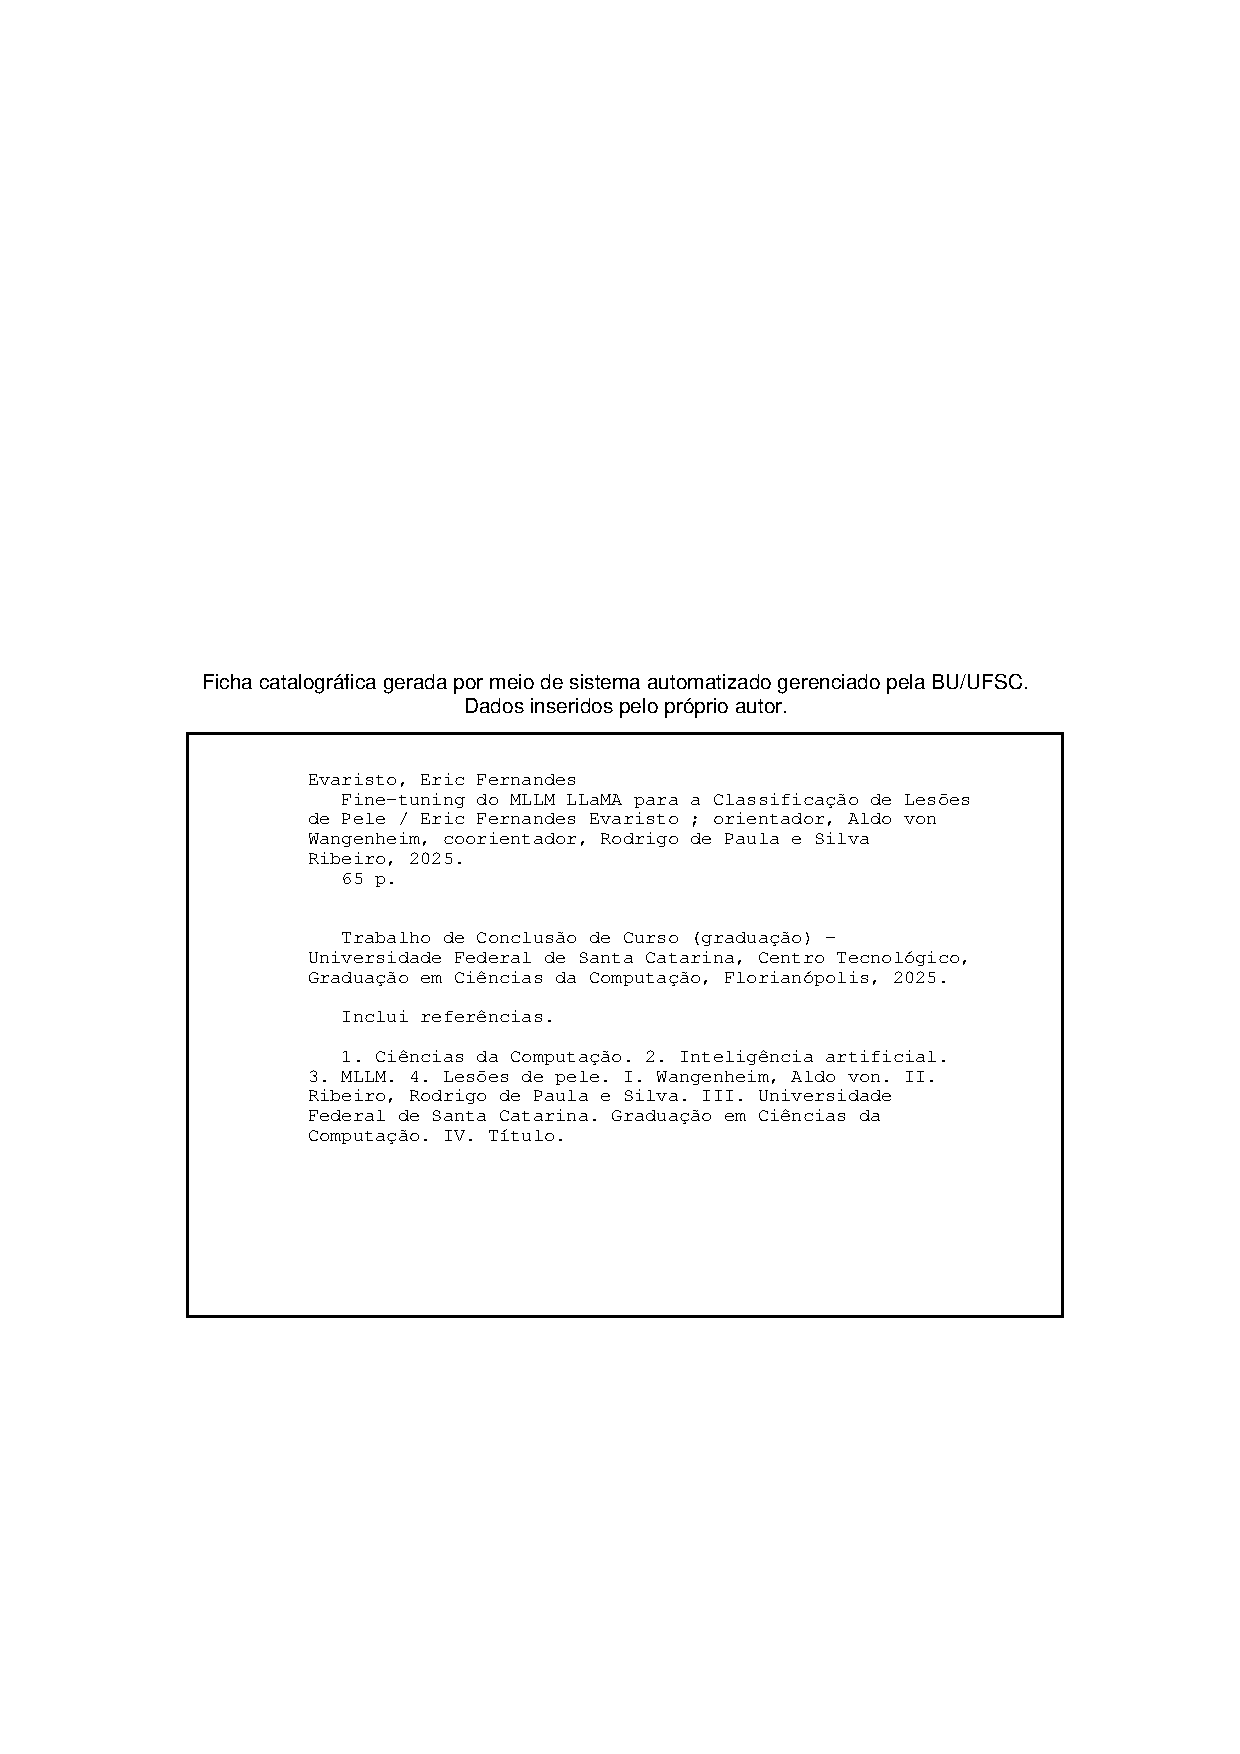
\includepdf{beforetext/Ficha_Catalografica.pdf}
\end{fichacatalografica}

% Folha de aprovação
\begin{folhadeaprovacao}
	\begin{center}
		{\imprimirautor}

		\begin{center}
			\ABNTEXchapterfont\bfseries\MakeUppercase{\imprimirtitulo}\ifnotempty{\imprimirsubtitulo}{: \imprimirsubtitulo}
		\end{center}

		\begin{minipage}{\textwidth}
			Este Trabalho de Conclusão de Curso foi julgado adequado para obtenção do Título de \imprimirformacao,
			e foi aprovado em sua forma final pelo Curso de Ciência da Computação.
		\end{minipage}%
	\end{center}

	\begin{center}
		\imprimirlocal, 15 de julho de 2025.
	\end{center}

	\assinatura{
		\textbf{\imprimircoordenador} \\
		Coordenação do Curso
	}

	\begin{center}
		\vspace{1cm}
		\textbf{Banca Examinadora:}
	\end{center}

	\vspace{1cm}
	\assinatura{
		\textbf{\imprimirorientador} \\ \imprimirorientadorRotulo
	}

	% \imprimircoorientador{
	% 	\assinatura{
	% 		\textbf{\imprimircoorientador} \\ \imprimircoorientadorRotulo \\
	% 		\imprimirinstituicao~--~\imprimirinstituicaosigla
	% 	}
	% }

	\vspace{1cm}
	\assinatura{
		\textbf{Prof. Convidado 1, Dr.} \\
		Instituição 1 -- Sigla 1
	}

	\vspace{1cm}
	\assinatura{
		\textbf{Prof. Convidado 2, Dr.} \\
		Instituição 2 -- Sigla 2
	}

	\begin{center}
		\vfill
		{
			\imprimirlocal\par
			\imprimirano\par
		}
	\end{center}
\end{folhadeaprovacao}

\begin{agradecimentos}
    ...
\end{agradecimentos}

% Resumo em português
\setlength{\absparsep}{18pt}
\begin{resumo}
	\SingleSpacing
	Lesões de pele podem ser um indicativo de diversas doenças, incluindo doenças graves como o câncer de pele. A detecção precoce dessas lesões é fundamental para o
	tratamento e cura da doença. Porém, o diagnóstico pode ser feito somente por profissionais qualificados, como dermatologistas.

	Uma parte do atendimento de atenção primária no Brasil é feita por \ac{ACS}. Esses profissionais estão em contato direto com a população, porém, eles não são
	qualificados para realizar a triagem de casos de lesões de pele. Considerando este cenário, uma ferramenta capaz de classificar lesões de pele e fornecer
	pré-diagnósticos pode ser útil.

	\acp{MLLM} possuem as capacidades necessárias para serem utilizados no desenvolvimento de uma ferramenta como esta, pois podem classificar imagens e gerar descrições
	textuais com base no seu conteúdo. Além disso, estes modelos podem ser treinados para tarefas específicas através de \textit{fine-tuning}.

	% TODO: Evidenciar mais o caráter experimental com "Com o objetivo de avaliar a possibilidade da utilização de um MLLM..."

	Neste trabalho, foi realizado o \textit{fine-tuning} do \ac{LLaMA} 3.2 para a classificação de lesões de pele e geração de laudos por meio das técnicas \ac{QLoRA} e
	\ac{LoRA}, ambas baseadas em \ac{PEFT}. Na etapa inicial dos experimentos, o conjunto de imagens de dermatoscopia \ac{HAM10000} foi utilizado para treinar o modelo
	para somente classificar lesões de pele, sendo que o melhor modelo resultante foi treinado com \ac{QLoRA} e obteve uma acurácia de 87,4\%. Para a etapa final,
	um conjunto de imagens de aproximação proveniente do \ac{STT/SC} foi utilizado no treinamento para a classificação de lesões e geração de laudos. O modelo final
	treinado com \ac{QLoRA} apresentou uma acurácia de 45,2\%, enquanto o modelo treinado com \ac{LoRA} obteve uma acurácia de 44,5\%. O baixo desempenho dos modelos finais
	pode ser explicado por inconsistências no conjunto de dados.

	\textbf{Palavras-chave}: Lesões de pele. Câncer de pele. MLLM. LLaMA. PEFT. Fine tuning. QLoRA. LoRA.
\end{resumo}

% Resumo em inglês
\begin{resumo}[Abstract]
	\SingleSpacing
	\begin{otherlanguage*}{english}
		Skin lesions can indicate various diseases, including serious diseases such as skin cancer. Early detection of these lesions is fundamental for treating and
		curing the disease. However, the diagnosis can only be made by qualified professionals, such as dermatologists.

		Some primary care in Brazil is provided by \acf{ACS}, or in English, community health workers. These professionals are in direct contact with the population, but
		they are not qualified to triage cases of skin lesions. Considering this scenario, a tool capable of classifying skin lesions and providing pre-diagnosis could be
		useful.

		\acfp{MLLM} possess the necessary capabilities to be employed in the development of a tool such as this, as they can classify images and generate textual descriptions
		based on their content. Furthermore, these models can be fine-tuned for specific tasks.

		In this work, the \acf{LLaMA} 3.2 model was fine-tuned for skin lesion classification and medical report generation using the \acf{QLoRA} and \acf{LoRA} techniques,
		both based on \acf{PEFT}. During the initial experimental phase, the \acf{HAM10000} dermatoscopy image dataset was used to train the model exclusively for skin lesion
		classification. The best-performing resulting model, trained with \ac{QLoRA}, achieved an accuracy of 87.4\%. For the final phase, a set of approximation images from
		the \acf{STT/SC} was utilized to train the model for both lesion classification and report generation. The final model trained with \ac{QLoRA} exhibited an accuracy
		of 45.2\%, while the model trained with \ac{LoRA} achieved an accuracy of 44.5\%. The low performance of the resulting models may be attributed to inconsistencies
		in the dataset.

		\textbf{Keywords}: Skin lesions. Skin cancer. MLLM. LLaMA. PEFT. Fine tuning. QLoRA. LoRA.
	\end{otherlanguage*}
\end{resumo}

{
\hypersetup{hidelinks}

% Lista de imagens
\pdfbookmark[0]{\listfigurename}{lof}
\listoffigures

% Lista de siglas
\imprimirlistadesiglas

% Sumário
\pdfbookmark[0]{\contentsname}{toc}
\tableofcontents*
\cleardoublepage
}
